\chapter{Experiments}

\section{Greedy Infomax model}
\begin{itemize}
	\item train CNN
	\item architecture: 4 layers ...
	\item dataset
\end{itemize}


\subsection{Dataset}
The Greedy Infomax model is trained on speech data. The model takes as input a raw speech signal of a fixed length and outputs a latent representation for that signal. The dataset is split up into 729 training files and 122 test files. In each file consists of a single spoken sound consisting of three consonants and three vowels, where the consonants and vowels alternate each other. Some Examples are the sounds "gi-ga-bu" and "ba-bi-gu". All the sounds are spoken by the same person, at a constant and peaceful \textbf{todo: describe emotional aspects of speech audio}. 

The following transformations are applied to the audio files. Although the original contains a sample rate of 441 Khz, the audio files are downsampled to 16 Khz, matching the sample rate used by Löwe \cite{lowePuttingEndEndtoEnd2020}. This significantly reduces the size of the latent representations, and thus the required amount of VRAM during training. Additionally, two types of noise are added to the data. We apply Gaussian white noise, at different decibels ranging between zero and fifteen \textbf{TODO ...}.

- also background noise from dataset. is a way to enlargen our dataset. 

%class RandomBackgroundNoise:
%def __init__(self, target_sample_rate, noise_dir, min_snr_db=0, max_snr_db=15):
%self.target_sr = target_sample_rate
%self.min_snr_db = min_snr_db
%self.max_snr_db = max_snr_db
%
%if not os.path.exists(noise_dir):
%raise IOError(f'Noise directory `{noise_dir}` does not exist')
%# find all WAV files including in sub-folders:
%self.noise_files_list = list(pathlib.Path(noise_dir).glob('**/*.wav'))
%if len(self.noise_files_list) == 0:
%raise IOError(
%f'No .wav file found in the noise directory `{noise_dir}`')

- Each audio file is cut to have length \textbf{10240}. Additionally, 


% split audio files into three separate files (one for each syllable)
Since the recordings are very consistent in loudness and are noise free, we can split up the files per syllable, obtaining three files per original sound (one for each syllable).

A sliding window is used of size 0.02 seconds. With a sample rate of 22050, this corresponds to roughly 500 samples per window. The maximum is computed for each window. Speech signals can then be split up when a severe dip happens in the signal. Regions where the amplitude is greater than 0.2 are considered \textbf{klinkers}, the regions with with lower values are considered \textbf{medeklinkers}. Apart from a few edge cases, this technique worked well enough for this purpose. In those cases, the splitting points closest to the one-third and two-third splitting points were considered.

\textbf{ERR: OUDE AFBEELDINGEN ZIJN WEG}
%\begin{figure}[h]
%	\centering
%	\includegraphics[width=0.7\linewidth]{"../../../../../../../../../GitHub/thesis-fabian-denoodt/GIM/datasets/gigabo/split up graphs/test/bababa_1"}
%	\caption{}
%	\label{fig:bababa1}
%\end{figure}
%
%\begin{figure}[h]
%	\centering
%	\includegraphics[width=0.7\linewidth]{"../../../../../../../../../GitHub/thesis-fabian-denoodt/GIM/datasets/gigabo/split up graphs/test/bababa_1_split"}
%	\caption{}
%	\label{fig:bababa1split}
%\end{figure}



note: we do need a hard threshold which is based on the signal's intentisity level. One could consider the alternative approach of looking at the gradient at each point and selecting the points with largest negative gradient. This will work in many cases, however, not for temporal envelops which gradually move towards zero, s.t: \ref{fig:example where gardient doesnt work}. Instead we use a dynamic threshold. This threshold is computed by creating transforming the signal into bins of 90'th percentile, creating a histogram of the single signal and applying otsu's image segmentation algorithm to obtain the threshold of that single audio sample.
We also tried directly applying otsu to the moving average and maximum of the bins. This either gave a threshold that was too small or too large. the 90th percent resulted in an acceptable compromise.


\begin{figure}[h]
	\centering
	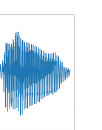
\includegraphics[width=0.7\linewidth]{screenshot011}
	\caption{}
	\label{fig:example where gardient doesnt work}
\end{figure}



Example where the explained strategy does not work: %\ref{fig:badadi1}
%\begin{figure}[h]
%	\centering
%	\includegraphics[width=0.7\linewidth]{"../../../../../../../../../GitHub/thesis-fabian-denoodt/GIM/datasets/gigabo/split up graphs/train/badadi_1"}
%	\caption{}
%	\label{fig:badadi1}
%\end{figure}/


Reference images for in the text:
\begin{figure}
	\centering
	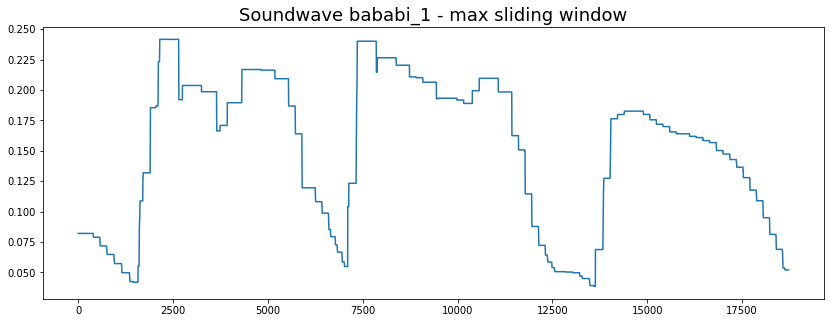
\includegraphics[width=0.7\linewidth]{screenshot012}
	\caption{}
	\label{fig:max sliding window}
\end{figure}

\begin{figure}
	\centering
	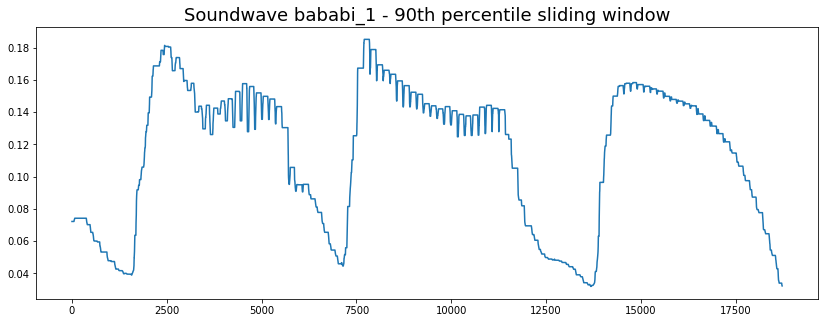
\includegraphics[width=0.7\linewidth]{screenshot013}
	\caption{}
	\label{fig:90th percentile}
\end{figure}

\begin{figure}
	\centering
	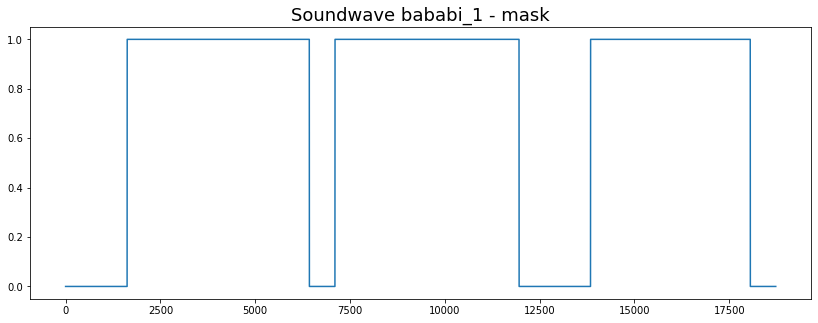
\includegraphics[width=0.7\linewidth]{screenshot014}
	\caption{}
	\label{fig:mask}
\end{figure}

\begin{figure}
	\centering
	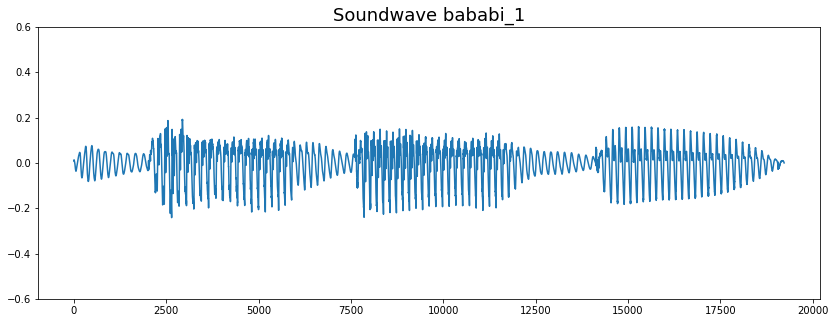
\includegraphics[width=0.7\linewidth]{screenshot017}
	\caption{}
	\label{fig:full sound wave adjusted yaxis}
\end{figure}


\begin{figure}
	\centering
	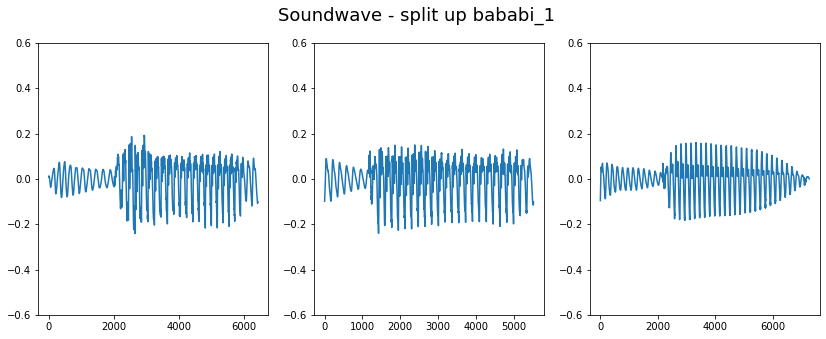
\includegraphics[width=0.7\linewidth]{screenshot016}
	\caption{}
	\label{fig:split up sound wave}
\end{figure}


\begin{figure}
	\centering
	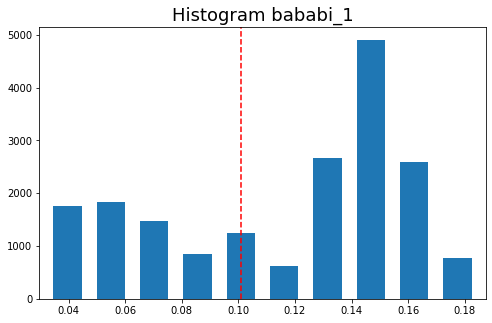
\includegraphics[width=0.4\linewidth]{screenshot018}
	\caption{}
	\label{fig:histogram}
\end{figure}


audio padded to maximum length. (added zeros in front and back)




\subsection{Training and validation during training}
Although loss is used as evaluation metric, it only shows part of the picture. The main objective for the representations is to obtain some form of "decoupled/dis-entanged" features that are more easily separable. This evaluation is done by projecting the latent representations to a 2D plane, via t-SNE.
Then datapoints are coloured in depending on their the syllable that was pronounced, eg: "gi" or "ga".

Training is done speech signals of fixed length, eg 8,800 samples. Notice however, that the neural network only makes use of convolutional neural networks layers and GRU's, no fully connected layers. The input dimensions can therefore be variable during inference. Only the number of channels in the latent representations should be constant, but the length can change.

During inference, (in this context obtaining the latent representations for our input signals), depending on the length of the input signal, the length of the output latent representation will differ.
If we wish to look at how separable latent representations are for syllables, the length can be variable. Some input sounds could be 6,600 samples, while others 8,800 samples. We therefore pad the syllables with zeroes in front and end of the signal, to obtain fixed length of equal to that of the longest syllable; 8,800 samples.

Training happens on longer data samples, and every \textbf{X} epochs t-SNE visualisations are made to observe evolutional of dis-entanglement.




\section{Decoders for Greedy Infomax}
Objective: understand GIM learned representations. To do so we first discuss the model's architecture. To verify whether GIM does in fact contain the necessary information, we reconstruct the original speech signal from a GIM representations. We define train a decoder model for each of the four layers of the GIM model.

\begin{itemize}
	\item Layer 1 ... 4
	\item Dataset from Bart
	\item Reduce audio to 16khz, reducing the size of the dataset and speeding up training time
	\item Add background noise to the data.
	\item Use this dataset: openslr.org instead of white noise as is more representative.
\end{itemize}






\section{Feature selection for visualisation}
The GIM architecture consists of 4 layers, each layer 512 kernels
Due to the large number of learned kernels, we filter based on standard deviation. This will result in looking at weights which are sensitive to particular features.


\section{Variational contrastive predictive coding}
\begin{figure}[h]
	\centering
	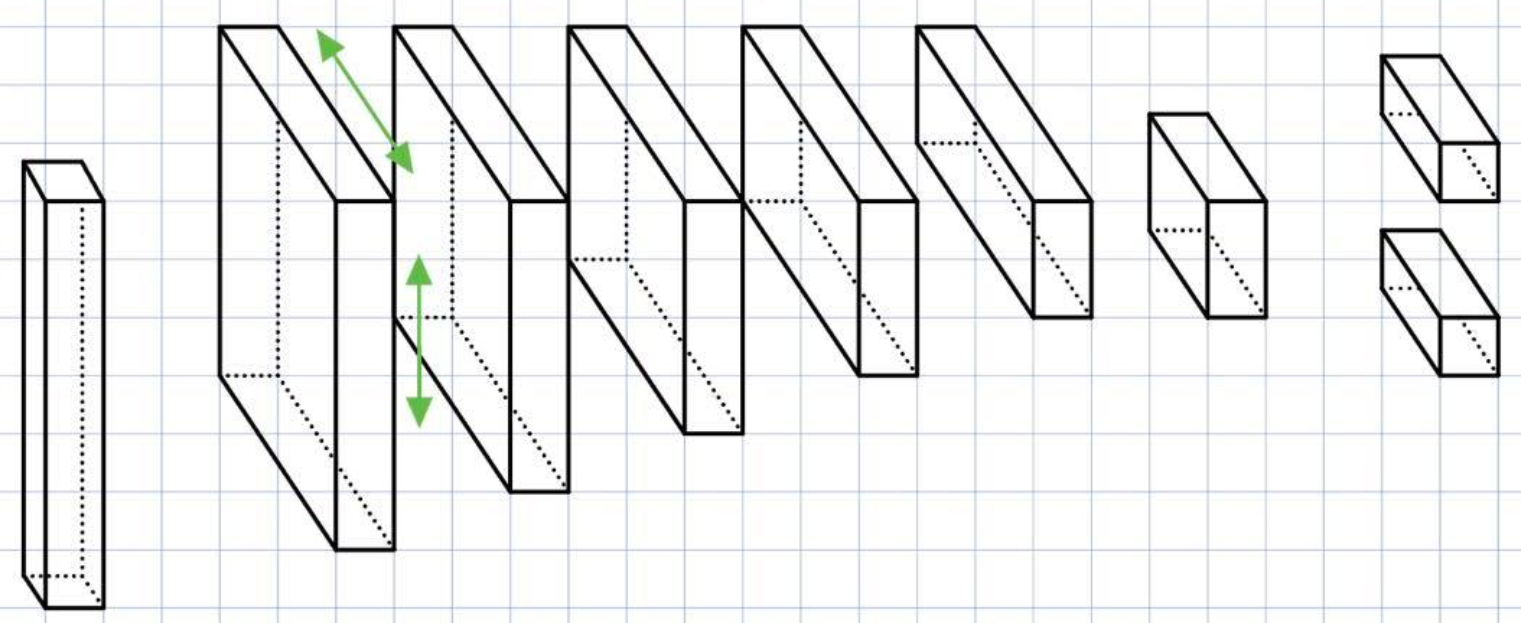
\includegraphics[width=0.7\linewidth]{architecture}
	\caption{}
	\label{fig:architecture}
\end{figure}
Figure \ref{fig:architecture} displays how via contrastive predictive coding an input speech signal is transformed into two latent vectors. The two vectors combined describe a Gaussian distribution for each feature of the latent representation. One vector corresponds to the means and the other to the standard deviations of the latent distributions. We variational autoencoders assume independent latent features, such that the covariance matrix is non negative on the diagonal and zero off the diagonal. This allows the covariance matrix to be discribed using a single vector. We again, make use of this (plausible incorrect?) assumption of having independent latent features.


\section{CHATGPT ANSWERS FOR VAE}
Yes, you can incorporate the regularization component from a VAE into the contrastive predictive coding (CPC) loss function to encourage the learned latent representations to be Gaussian distributed. This can be achieved by adding a KL divergence term between the learned latent distribution and a Gaussian prior distribution to the CPC loss function.

The modified loss function would be:

\begin{equation}
	\mathcal{L}{N+KL} = - \sum{k} \mathbb{E}{\textsubscript{X}} \left[ log \frac{f_k(z{t+k}, c_t)}{\sum_{z_j \in X} f_k(z_j, c_t)} \right] + \lambda \text{KL}(q(z|X) || \mathcal{N}(0, I))
\end{equation}

where $q(z|X)$ is the learned distribution of latent representations, and $\mathcal{N}(0, I)$ is the standard Gaussian prior distribution. The hyperparameter $\lambda$ controls the weight of the KL divergence term in the overall loss function.

To compute the KL divergence term, we need to calculate the mean and covariance of the learned latent distribution $q(z|X)$. Let $\mu$ and $\Sigma$ be the mean and covariance of $q(z|X)$, respectively. Then the KL divergence can be computed as:

\begin{equation}
	\text{KL}(q(z|X) || \mathcal{N}(0, I)) = \frac{1}{2} \left( \text{tr}(\Sigma) + \mu^T \mu - k - \log \det(\Sigma) \right)
\end{equation}

where $k$ is the dimensionality of the latent space.

The function $f_k(z_j, c_t)$ can be defined using a linear layer as follows:

\textbf{code}
%W_k = torch.nn.Linear(hidden_size, latent_size, bias=False)
%f_k = lambda z, c: torch.exp(torch.matmul(W_k(z), c.T))

Here, `hidden size` is the size of the hidden layer, `latent size` is the size of the latent space, and c is the context vector for a given time step. The function $W_k(z)$ applies a linear transformation to the input z, resulting in a latent vector of size `latent size`.

To incorporate the KL divergence term into the CPC loss function, you can compute the mean and covariance of the learned latent distribution using the torch.mean and torch.var functions, respectively. The modified loss function can then be implemented as follows:

\textbf{code}
%def cpc_loss_with_regularization(z, c, lambd):
%# Compute the CPC loss
%logits = compute_logits(z, c)
%cpc_loss = -torch.mean(torch.log_softmax(logits, dim=-1)[:, 0])
%
%# Compute the mean and covariance of the learned latent distribution
%mu = torch.mean(z, dim=0)
%sigma = torch.var(z, dim=0)
%
%# Compute the KL divergence loss
%kl_loss = 0.5 * (torch.sum(sigma) + torch.matmul(mu, mu.T) - mu.shape[0] - torch.log(torch.prod(sigma)))
%
%# Compute the total loss
%loss = cpc_loss + lambd * kl_loss
%
%return loss

Here, z is the learned latent representation, c is the context vector, and lambd is the weight of the KL divergence term. The `compute logits` function computes the logits for the CPC loss as described in the original CPC paper.

Note that this implementation assumes that the ....

---


To incorporate the regularization component from VAE into the CPC loss function, we can add the Kullback-Leibler (KL) divergence term to the loss function, which will encourage the latent representations to be Gaussian distributed. The KL divergence term measures the difference between the learned latent distribution and the target Gaussian distribution.

The KL divergence term can be defined as:

$$\mathcal{L}{KL} = \frac{1}{2}\sum{i=1}^d (\mu_i^2 + \sigma_i^2 - \log(\sigma_i^2) - 1)$$

where $\mu_i$ and $\sigma_i$ are the mean and standard deviation of the $i$-th dimension of the learned latent distribution, and $d$ is the dimension of the latent space.

To combine the CPC loss and the KL divergence term, we can simply add them together, with a weighting factor $\beta$ to balance their contributions:

$$\mathcal{L} = \mathcal{L}N + \beta\mathcal{L}{KL}$$

where $\mathcal{L}_N$ is the CPC loss function defined in equation (\ref{eq:NCE_loss}), and $\beta$ is a hyperparameter that controls the strength of the regularization term.

The final loss function will encourage the learned latent representations to be both informative for the CPC task and Gaussian distributed, which can be useful for downstream tasks such as clustering or classification.



---

Sure! In the context of contrastive predictive coding (CPC), the `compute logits` function is used to compute the similarity scores (logits) between the predicted future and the actual future.

In more detail, `compute logits` takes in two inputs, z and c, which represent the latent representation and the context for a given time step, respectively. The function computes the similarity score between the predicted future representations and the actual future representations by performing a dot product between the predicted future representation and a set of parameters (i.e., weights) that are learned during training. Specifically, `compute logits` applies a linear transformation to the context c and uses it to score each element in the predicted future z.

The output of `compute logits` is a vector of logits that corresponds to the similarity scores between each predicted future representation and the actual future representation. These logits are then used to compute the contrastive loss, which is a measure of the similarity between the predicted future and the actual future.

The `compute logits` function is a crucial component of the CPC algorithm, as it determines how well the predicted future representations match the actual future representations, which in turn affects the quality of the learned latent representation.




\section{Results}
% Enkele loss curces etc
\subsection{Results CPC Simple v2 w/ 2 modules}

\begin{figure}[h]
	\centering
	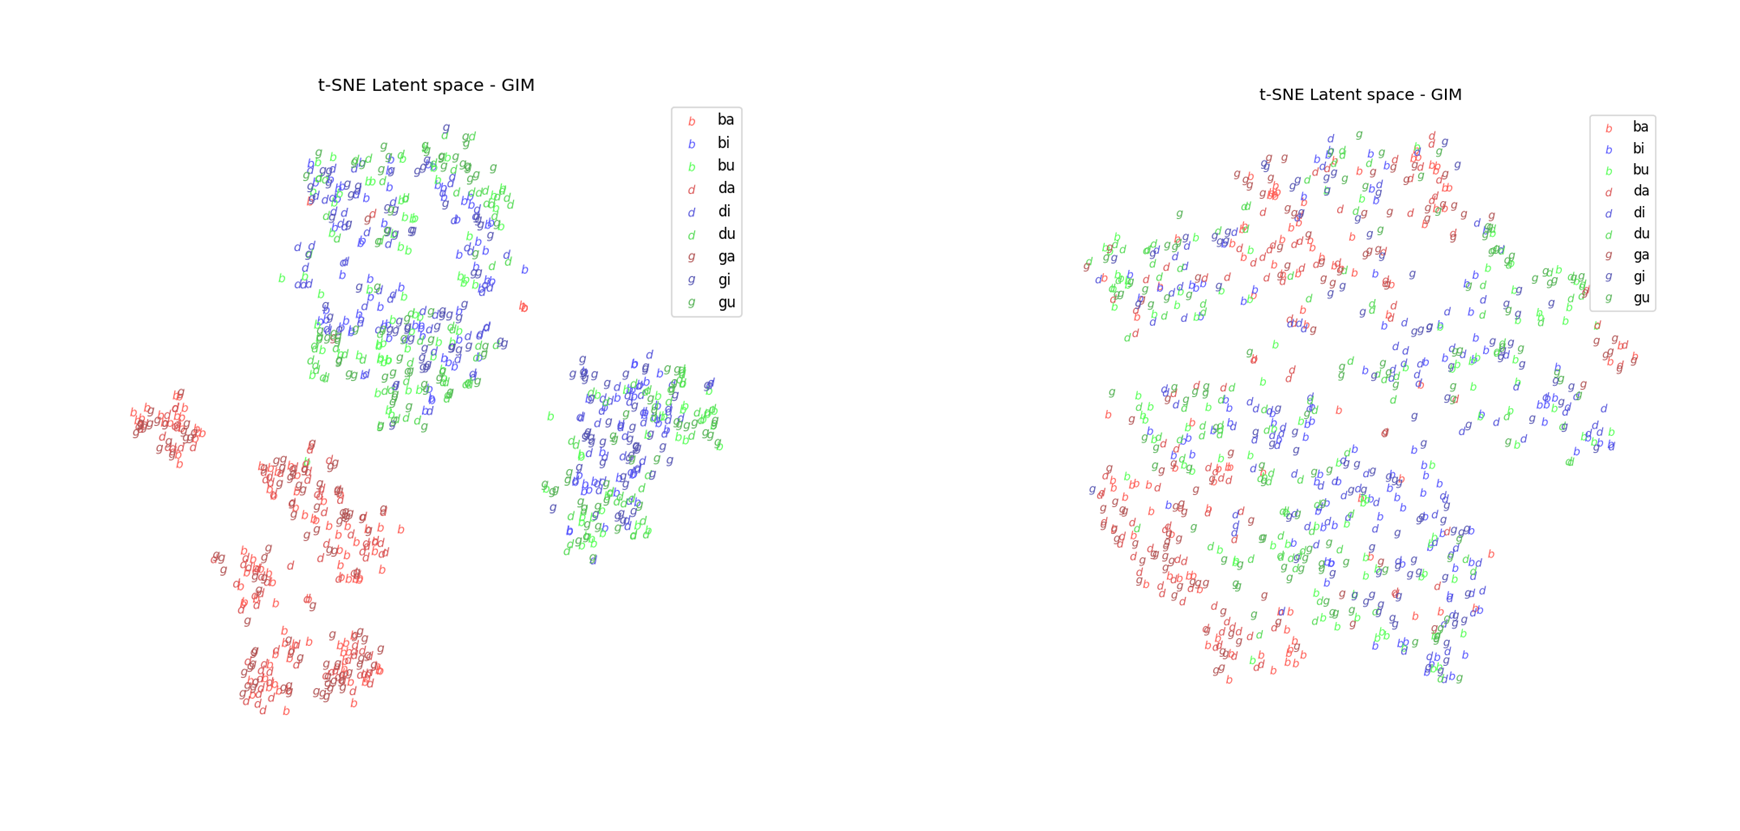
\includegraphics[width=0.7\linewidth]{screenshot023}
	\caption{}
	\label{fig:tsne_two_module_kld_0}
\end{figure}


\begin{figure}[h]
	\centering
	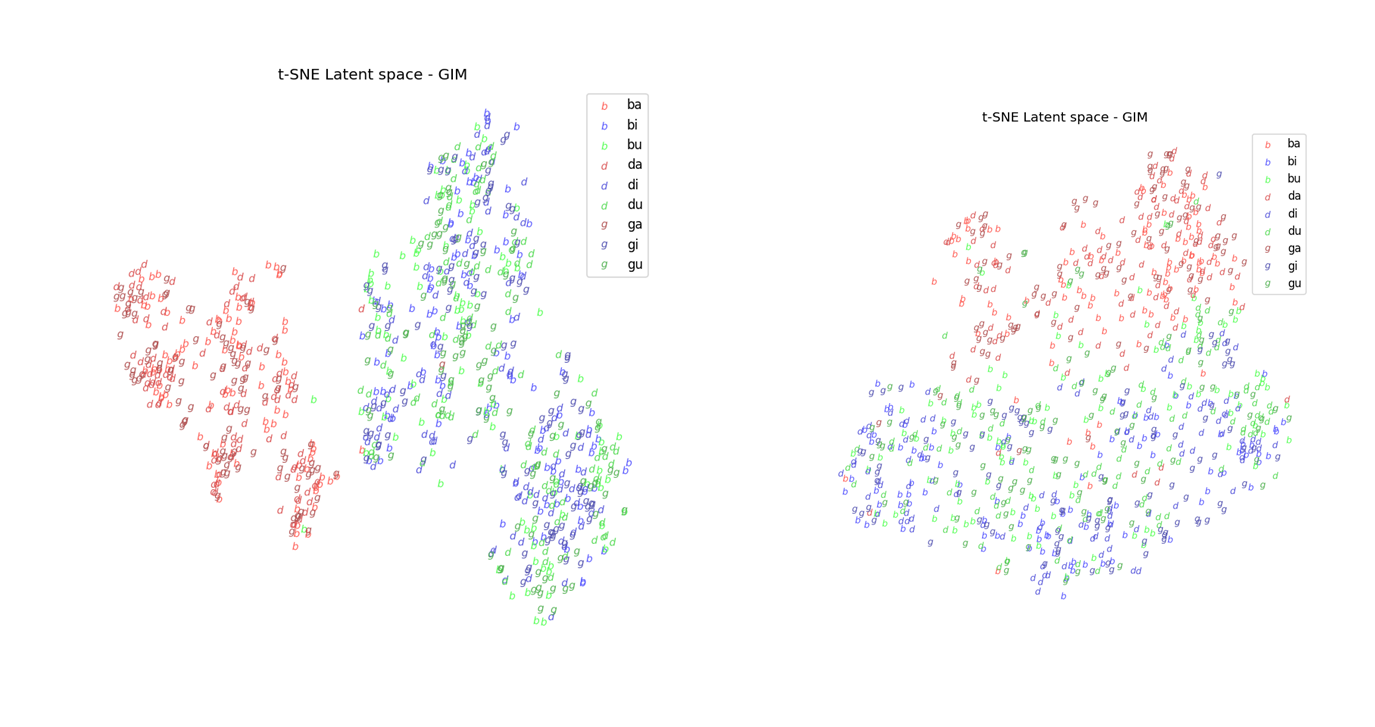
\includegraphics[width=0.7\linewidth]{screenshot024}
	\caption{}
	\label{fig:tsne_two_module_kld_0033}
\end{figure}

\ref{fig:tsne_two_module_kld_0}: can see that second model harms performance. We believe this can be explained via the learning rate. \ref{fig:tsne_two_module_kld_0033}, there we see that second module performs better separation, indicating that the intermediate KL convergence constraint (causing the normal Gaussian distributions) also serves as a batch normalisation term, and thus resulting in faster convergence.




\section{GIM: Activations visualisations}

%these were notes from the decoder from file: eval_autoencoder.py
thought for later: its actually weird i was able to play enc as audio as enc is 512 x something
so huh? that means that a lot of info is already in first channel? what do other 511 channels then contain?
"""
Observations:
First layer decoded still contains the same sound, but with some added noise (could be because decoder hasn't trained very).
However, the encoded first layer, still contains the exact sound as the original sound. It is however downsampled a lot -> from 16khz to ~3khz
"""
thought for later: its actually weird i was able to play enc as audio as enc is 512 x something
so huh? that means that a lot of info is already in first channel? what do other 511 channels then contain?



\begin{figure}[h]
	\centering
	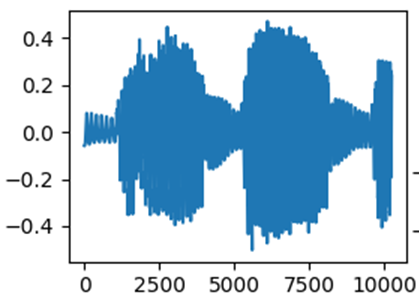
\includegraphics[width=0.7\linewidth]{screenshot007}
	\caption{"BA-BA-BA" time domain}
	\label{fig:screenshot007}
\end{figure}

\begin{figure}[h]
	\centering
	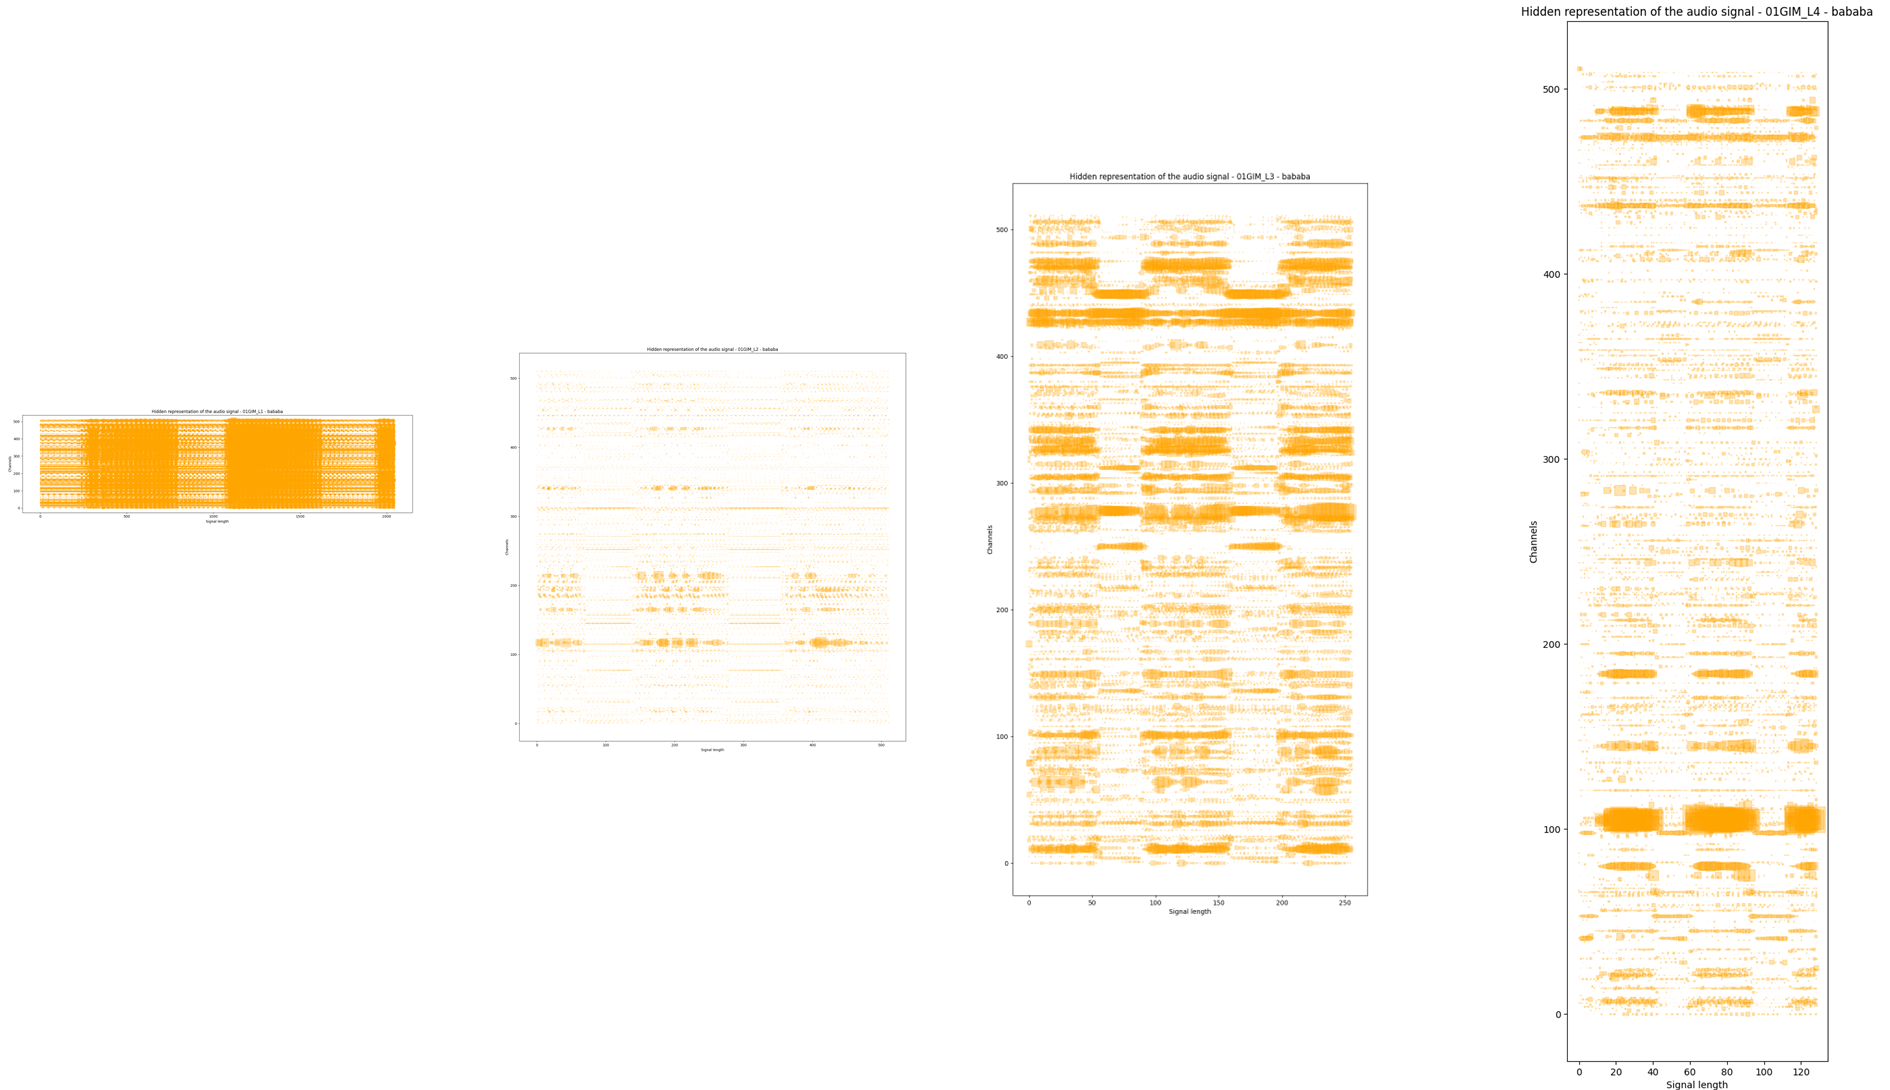
\includegraphics[width=0.7\linewidth]{screenshot006}
	\caption{Activations of the sound "BA-BA-BA" through GIM}
	\label{fig:gim latent activations}
\end{figure}

No batch normalisation, so although channels appear to have larger activations than other channels, size of activation does not really say anything about information. eg activations 0.01 could still contain more information than 3.0 activation.

Since the activations from convolutional neural networks, the order is still maintained. Hence, can align activations with original signal.

Observations in latent representations:

\textit{Layer 1:}
The activations of the first decoder still contain a lot of similarity with the original signal, in terms of structure. There is a lot of redundant data within the representation. Eg: the one channel could be replied 

Layer 2

Layer 3:

Layer 4:
Still notices multiple channels which have high activations when signal is has high amplitudes and small activations when amplitude is low. 

Also activations which are high when volume is low. --> indicates that certain kernel weights are sensitive for \textbf{"klinkers"} and other kernels for \textbf{medeklinkers}. see \ref{fig:screenshot008}.

\begin{figure}[h]
	\centering
	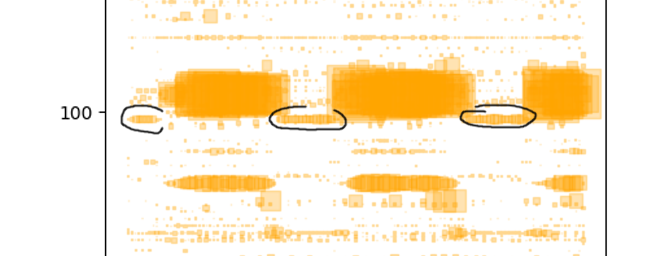
\includegraphics[width=0.7\linewidth]{screenshot008}
	\caption{zoomed in}
	\label{fig:screenshot008}
\end{figure}


Observe that activations happen in clusters/sequences. So it is usually a patch of signal samples that cause high activations. This could for instance indicate that both kernels are sensitive for the \textbf{medeklinker} "b", but sensitive for different features. eg the letter B has spoken sound "buh". so maybe one is sensitive for "b" and other for "uh".

Figure \ref{fig:layer4 zoomed in} also nicely shows how different channels have clusters of activations at slightly different times. 

\begin{figure}[h]
	\centering
	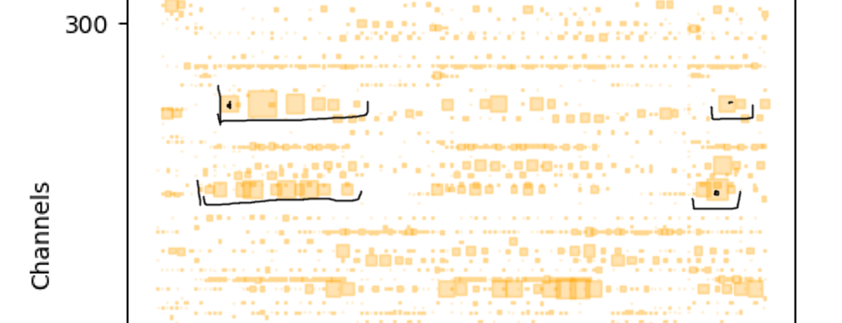
\includegraphics[width=0.7\linewidth]{screenshot010}
	\caption{Zoomed in}
	\label{fig:layer4 zoomed in}
\end{figure}



---------------------------------------------

\textbf{T-sne visualisations:}
Multiple models trained, trained GIM, but single module (exact CPC architecture), one with autoregressor and once without autoregressor layer, so only CNN layers. 200 epochs, trained on split up data samples.

1) Only CNN: We observe better linear separability
\begin{figure}[h]
	\centering
	\includegraphics[width=0.7\linewidth]{"cpc architecture ONLY CNN t-SNE_latent_space_GIM"}
	\caption{}
	\label{fig:cpc-architecture-only-cnn-t-snelatentspacegim}
\end{figure}

2) CNN + 1 autoregressor layer:
\begin{figure}[h]
	\centering
	\includegraphics[width=0.7\linewidth]{"cpc architecture CNN + GRU t-SNE_latent_space_GIM"}
	\caption{}
	\label{fig:cpc-architecture-cnn--gru-t-snelatentspacegim}
\end{figure}

3) This is the pure data visualised (no latent representation).
Were at least doing a bit better than the original data, so that's good! our work is not for nothing.
\begin{figure}[h]
	\centering
	\includegraphics[width=0.7\linewidth]{"_ t-SNE_latent_space_Original data"}
	\caption{}
	\label{fig:-t-snelatentspaceoriginal-data}
\end{figure}


4) old GIM with all modules each one layer. l1 .. 5 - cnn, l6 = gru. img shows l5 = cnn:
model can more easily distinguish A's from other \textbf{klinkers}. Partly, it kinda makes sense for GIM to learn to separate \textbf{klinkers}. Since they last longer (longer duration), the loss function will more likely randomly sample a subwindow from the "aa's" than from the \textbf{medeklinker} part.


\begin{figure}[h]
	\centering
	\includegraphics[width=0.7\linewidth]{"_ t-SNE_latent_space_GIM multi module cnn layer 5"}
	\caption{}
	\label{fig:-t-snelatentspacegim-multi-module-cnn-layer-5}
\end{figure}
% 	







\section{Decoder: predictions on test set}
Fig \ref{fig:bagidi1-model29-true-vs-predicted} displays the reconstructed signal from the vocal sound "ba-gi-di". The two images on the left displays the original signal, while the right two images contain the reconstructed signal.  The upper images displays the signals in time domain, the bottom images spectral domain. The reconstructed signal is an audio sample, for instance which is encoded via Greedy Infomax (up to the fourth (and final) convolution layer), this output is then given to a decoder to reconstruct the original signal.

%TODO: BROKE 
%\begin{figure}[h]
%	\centering
%	\includegraphics[width=0.7\linewidth]{"../../../../../../../../../GitHub/thesis-fabian-denoodt/GIM/logs/GIM_DECODER_experiment/MSE + scFFT Loss FFT=10240 Lambda=1.0000000/lr_0.0010000/GIM_L4/predictions_model=29/test/bagidi_1, model=29, True vs Predicted"}
%	\caption{Top left: original, time domain. Bottom left: original }
%	\label{fig:bagidi1-model29-true-vs-predicted}
%\end{figure}


